\section{\textbf{METODOLOGÍAS ÁGILES}}
		En febrero de 2001, tras una reunión celebrada en Utah - EEUU, nace el término “ágil” aplicado al desarrollo de software. En esta reunión participan un grupo de 17 expertos de la industria del software, incluyendo algunos de los creadores o impulsores de metodologías de software. Su objetivo fue esbozar los valores y principios que deberían permitir a los equipos desarrollar software rápidamente y respondiendo a los cambios que puedan surgir a lo largo del proyecto. Se pretendía ofrecer una alternativa a los procesos de desarrollo de software tradicionales, caracterizados por ser rígidos y dirigidos por la documentación que se genera en cada una de las
		actividades desarrolladas.\vspace*{0.3in}
		
		Tras esta reunión se creó The Agile Alliance 3 , una organización, sin ánimo de lucro, dedicada a promover los conceptos relacionados con el desarrollo ágil de software y ayudar a las organizaciones para que adopten dichos conceptos. El punto de partida es fue el Manifiesto Ágil,
		un documento que resume la filosofía “ágil”.\vspace*{0.3in}
		
		Según el informe de Standish, las diez causas principales de los fracasos, por orden de importancia, son:\vspace*{0.3in}
		
		\begin{table}[htbp]
			\centering
			\begin{tabular}{|c|c|}
				\hline
				\rowcolor[HTML]{9B9B9B} 
				\textbf{Ítem} & \textbf{Causas de fracaso}                                  \\ \hline
				1             & Escasa participación de los usuarios                        \\ \hline
				2             & Requerimientos y especificaciones incompletas               \\ \hline
				3             & Cambios frecuentes en los requerimientos y especificaciones \\ \hline
				4             & Falta de soporte ejecutivo                                  \\ \hline
				5             & Incompetencia tecnológica                                   \\ \hline
				6             & Falta de recursos                                           \\ \hline
				7             & Expectativas no realistas                                   \\ \hline
				8             & Objetivos poco claros                                       \\ \hline
				9             & Cronogramas irreales                                        \\ \hline
				10            & Nuevas tecnologías                                          \\ \hline
			\end{tabular}
			\caption{Causas principales de fracasos.}
			\label{}
		\end{table}
			\begin{figure}
				\centering
				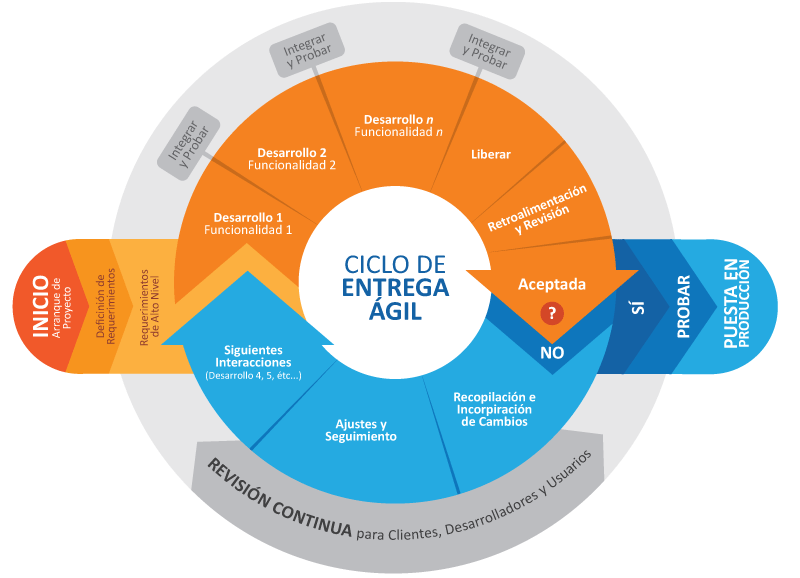
\includegraphics[width=0.7\linewidth]{graficos/agile}
				\caption{Ciclo de entrega ágil}
				\label{fig:agile}
			\end{figure}
			